% Vasa nations sångbok Vasungavisor 2018

\documentclass[a6paper,8pt,makeidx,openany]{book}
\usepackage[a6paper]{geometry}
\usepackage[T1]{fontenc}
\usepackage[utf8]{inputenc} %UTF8 stöd så att jag kan skriva åäö
\usepackage[swedish]{babel}
\usepackage{fancyhdr}
\usepackage[pdftex]{graphicx}	% Kuvat kyttn, tukee .png, .jpg ja .pdf-kuvia
\usepackage{import}		% Verbatim-tekstityyppi
\usepackage{setspace}
\usepackage[lyric]{songs}
\usepackage{graphicx,eso-pic}

% Sidnummer samt header/footer
\pagestyle{empty}

% Antal kolumner
\songcolumns{1}

% Sätter in ett extra avstånd på 5mm efter varje sång
\renewcommand{\extendpostlude}{
  \vspace{3mm}
}

% Tjockleken på skiljelinjen mellan sångerna
\setlength{\sbarheight}{0pt}

% Tjockleken på linjen framför refrängen
\setlength{\cbarwidth}{1pt}

% Storleken på texten
\renewcommand{\lyricfont}{\footnotesize}

% Storleken på rubrikerna
\renewcommand{\stitlefont}{\sffamily\large}

% Hindrar sångerna från att stretcha över hela sidan
\renewcommand{\colbotglue}{0pt plus .5\textheight minus 0pt}

% Bakgrundsfärgen på låtnumrering och sångkommentarer
\definecolor{bgshade}{RGB}{235,235,235}
\renewcommand{\snumbgcolor}{bgshade} % låtnumrering
\renewcommand{\notebgcolor}{bgshade} % sångkommentarer

% Inga nummer på verserna
\noversenumbers

% Skapa register med namnet 'titleidx' för filerna
\newindex{titleidx}{titleidx}

\newcommand\chapterimage[2][]{%
  \AddToShipoutPictureBG*{% Add picture to BackGround on this page only
    \AtTextLowerLeft{% Position at lower left of text block
      \hspace*{.85\textwidth}% Move over to the right of text block
      \llap{% Ignore horizontal width and overlap to the left
        \smash{% Ignore vertical height
          \raisebox{.1\textheight}{%
            \includegraphics[#1]{#2}}}}}}}% Include image with options

\begin{document}
\import{./Uppslag/}{uppslag.tex}
%\import{./Uppslag/}{innehall.tex}

\begin{songs}{titleidx}
\import{./Forord/}{forord.tex}

\import{./IHoganNord/}{inord.tex}
\sclearpage

\import{./IUngdomensVar/}{ungdom.tex}
\sclearpage

\import{./UrTorstigaStrupar/}{strupar.tex}	
\sclearpage

\import{./SaHarligBouquet/}{bouquet.tex}	
\sclearpage

\import{./ArrakAckJa/}{arrak.tex}	
\sclearpage

\import{./KunBotnialleSisaanAstuu/}{botnia.tex}	
\sclearpage

\import{./FafaSkaSjung/}{fafa.tex}	
\sclearpage

\import{./AuldAcquaintance/}{auld.tex}	
\sclearpage

\import{./BlomdoftIMelodin/}{blomdoft.tex}
\sclearpage

\import{./Silliskapitel/}{sillis.tex}
\sclearpage

\import{./VettOchEtikett/}{vett.tex}
\sclearpage


\end{songs}
\begin{figure}[h]
	\begin{center}
		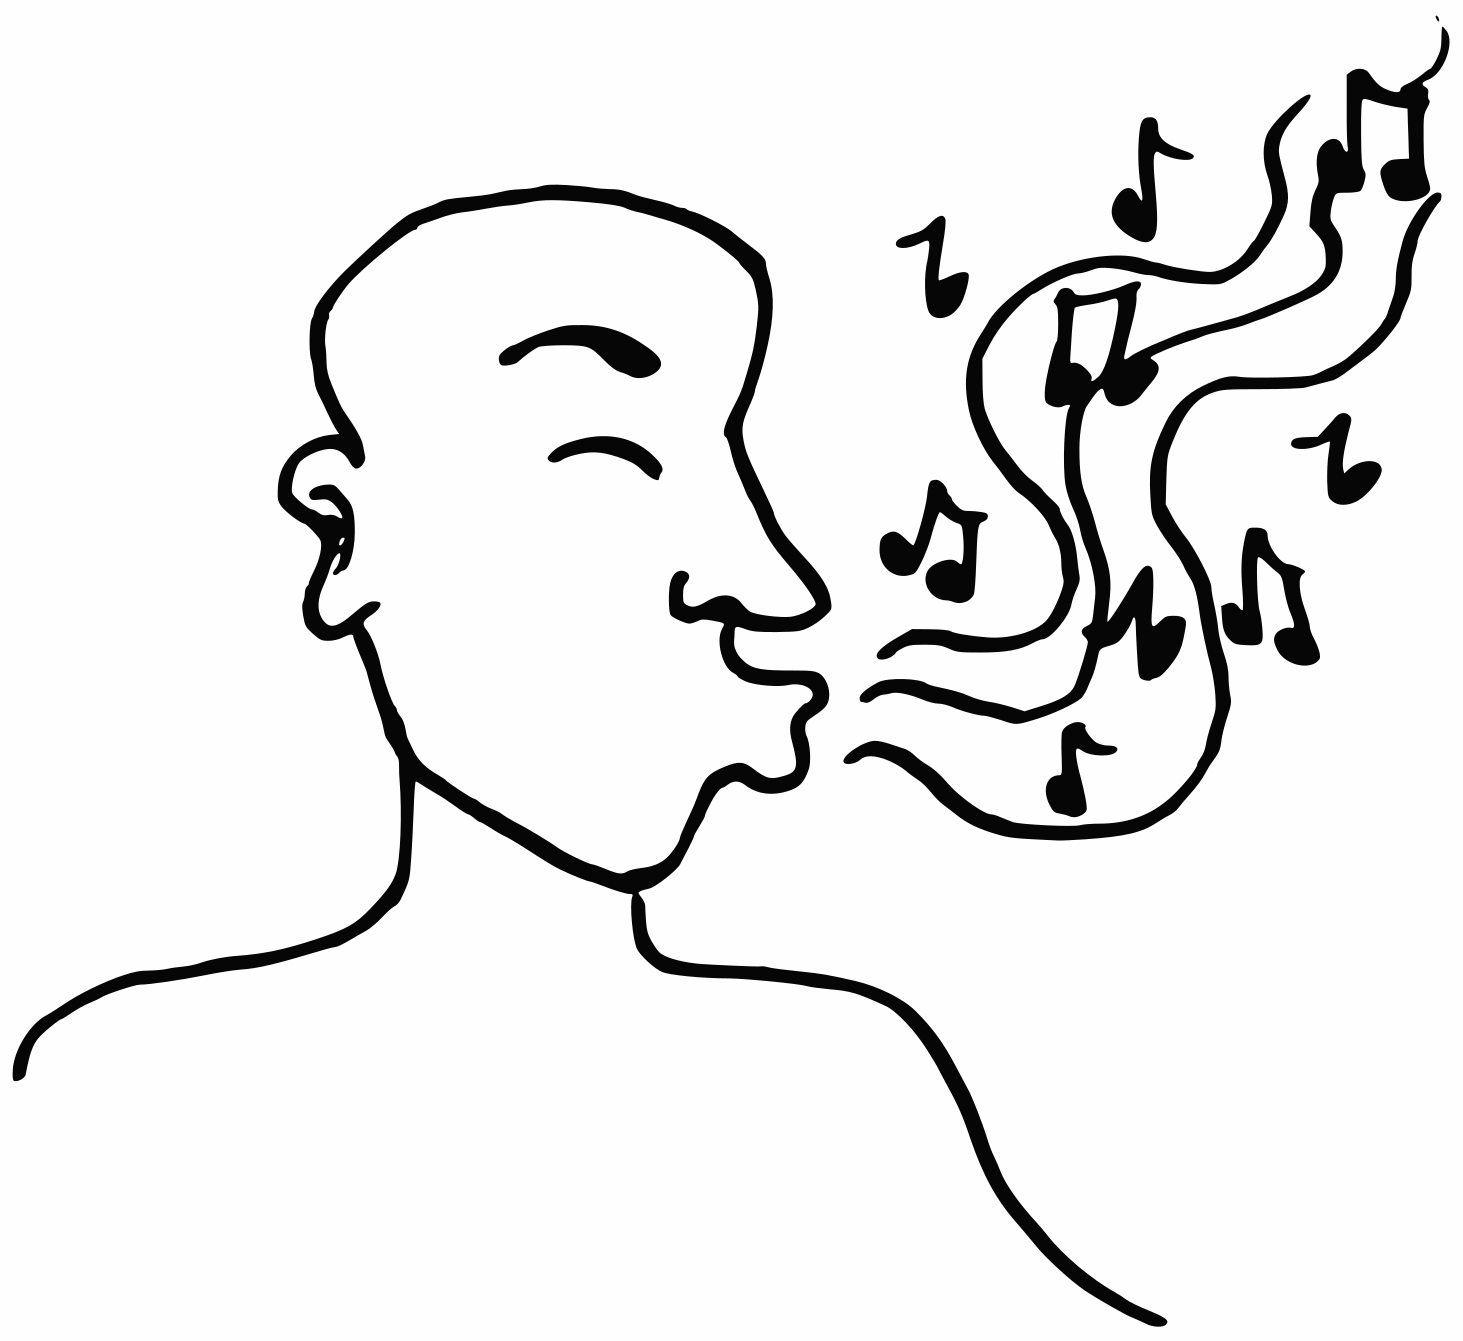
\includegraphics[width=40mm]{./bilder/fardigabilder/BilderTillKapitel/visslaren.png} 
	\end{center}
\end{figure}
% Registrets utseende
\renewcommand{\idxtitlefont}{\rmfamily\mdseries}
\renewcommand{\idxlyricfont}{\rmfamily\mdseries}
\renewcommand{\idxheadfont}{\sffamily\it\large}
\setlength{\idxheadwidth}{0.5cm}
\showindex{Register}{titleidx}
\end{document}